% пятая часть

\section{Разработка мобильного приложения}

\subsection{Разработка концепции и архитектуры мобильного приложения, предназначенных для преобразования 2D в 3D}
В ходе выполнения работы были рассмотрены различные варианты для создания мобильных приложений, предназначенных для преобразования 2D изображений в 3D вид. При этом рассмотрении учитывалось, что результирующие мобильные приложения должны создаваться под операционные системы Android и iOS, а также то, что один из основных результатов работы приложения с точки зрения конечного пользователя – это возможность публикации созданного 3D-изображения в виде анимированного gif-файла в одном или нескольких аккаунтов в социальных сетях пользователя. Соответственно, можно исходить из предположения о том, что для функционирования приложения в любом случае необходим доступ к сети интернет. Максимальная унификация различных составных частей приложения между собой хотя бы на уровне исходных кодов вне зависимости от целевой платформы (Android или iOS) является дополнительным преимуществом при рассмотрении различных вариантов создания мобильных приложений.

Один из наиболее простых с технической точки зрения вариантов реализации решения, позволяющего преобразовывать 2D файлы в 3D вид, является решение, основанное на создании веб-сервиса, который предоставляет минимально необходимый пользовательский интерфейс для загрузки желаемого файла на сервер, преобразования файла на сервере и, как результат, возможность скачать получившийся файл на устройство пользователя и поделиться этим файлом в социальных сетях. При простоте архитектуры у этого решения есть один существенных недостаток – как правило, такие решения менее удобны и функциональны, чем нативные (native) мобильные приложения, разработанные специально под целевую платформу, на которой они будут функционировать. Поэтому на данном этапе от такого подхода было принято решение отказаться.

Если рассматривать варианты создания нативных мобильных приложений, существует несколько возможных вариантов:

\begin{enumerate}
	\item Использовать наиболее популярные средства разработки и языки программирования для каждой из необходимых мобильных платформ. Создать нативное мобильное приложение, реализующее весь необходимый пользовательский интерфейс, набор сервисных функций. Портировать алгоритм преобразования графического файла из 2D в 3D для локального исполнения на мобильном устройстве. Все необходимые преобразования выполнять локально, на мобильном устройстве. Полученный результат преобразования (анимированный gif) загружать в интернет (социальные сети) по мере его готовности на мобильном устройстве.
	\item Использовать наиболее популярные средства разработки и языки программирования для каждой из необходимых мобильных платформ для создания нативных мобильных приложений только для реализации пользовательского интерфейса и набора сервисных функций. Алгоритм преобразования графического файла из 2D в 3D реализуется в виде серверного модуля, соответственно для преобразования выбранного файла и предварительного просмотра полученных результатов необходимо загрузить этот выбранный файл на сервер. Загрузить полученный результат с сервера и поделиться этим результатом в социальных сетях.
	\item Использовать кроссплатформенное средство разработки мобильных решений Xamarin. Это средство одновременно позволяет создавать iOS, Android и Windows Phone приложения. Реализация алгоритма преобразования графического файла из 2D в 3D модифицируется таким образом, что может быть непосредственно интегрирована в Xamarin-проект. В результате получается единое решение, которое на этапе сборки может быть превращено в полнофункциональное нативное приложение для любой из поддерживаемых платформ --- iOS, Android и Windows Phone. Результирующее решение будет преобразовывать графические файлы из 2D в 3D локально на мобильном устройстве, доступ к интернету необходим только для реализации функции «поделиться созданным 3D-файлом в социальных сетях».
	\item Использовать кроссплатформенное средство разработки мобильных решений Xamarin, но только лишь для создания нативных мобильных приложений. реализующих пользовательский интерфейс и набор сервисных функций. Алгоритм преобразования графического файла из 2D в 3D реализуется в виде серверного модуля, соответственно для преобразования выбранного файла и предварительного просмотра полученных результатов необходимо загрузить этот выбранный файл на сервер. Загрузить полученный результат с сервера и поделиться этим результатом в социальных сетях.
\end{enumerate}

Перед тем, как рассмотреть каждый из приведенных выше вариантов по отдельности, следует отметить, что существующая на сегодняшний день реализация алгоритма преобразования изображений из 2D в 3D вид реализована на языке С++, сборка осуществляется с использованием Microsoft Visual Studio, соответствующее решение имеет существенную зависимость от OpenCV (Open Source Computer Vision Library – это программная библиотека с открытым исходным кодом, реализующая базовые алгоритмы компьютерного зрения, обработки изображений и численных алгоритмов общего назначения. Реализована на C/C++).

Возвращаемся к вышеперечисленным вариантам.

Для варианта №1 для операционной системы Android необходимо:

С использованием Android Studio на языке программирования Java реализовать необходимый пользовательский интерфейс, а также весь необходимый набор сервисных функций. Необходимо адаптировать реализацию алгоритма преобразования графического файла из 2D в 3D для использования под управлением операционной системы Android (реализация на С++). Далее, с использованием механизма The Android Native Development Kit (NDK) необходимо обеспечить вызов кода, написанного на языке С++ из «классического» Android-приложения. 

Для разработки приложений для iOS основным средством разработки является Objective-C. Проведенные предварительные исследования показали, что адаптировать реализацию алгоритма преобразования графического файла из 2D в 3D для использования под управлением операционной системы iOS с разумными усилиями не представляется возможным. Соответственно, вариант №1 является неприемлемым для реализации решения для операционной системы iOS.

Для реализации варианта №2 необходимо:

С использованием наиболее популярных средств разработки и языков программирования для каждой из необходимых мобильных платформ (Java для Android и Objective С для iOS) необходимо создать нативные мобильных приложений для реализации пользовательского интерфейса и набора сервисных функций. Эта задача, в целом, является типовой и принципиальных сложностей не вызывает. Алгоритм преобразования графического файла из 2D в 3D следует реализовать в виде серверного модуля, например, для использования под управлением операционной системы Ubuntu. Это обусловлено тем, что Unix-подобные операционные системы имеют существенно более широкое распространение в Web-серверном окружении, чем Windows-сервера. Основная сложность данной задачи – в сборке и корректном использовании OpenCV библиотеки под Linux, однако аналогичная задача сравнительно недавно была решена коллегами для реализации демонстрационного видеоплеера для использования под операционной системой Ubuntu.

Для реализации варианта №3 необходимо адаптировать алгоритм преобразования графического файла из 2D в 3D таким образом, чтобы он мог быть непосредственно интегрирован в Xamarin-проект (разработка на языке программирования С\#). Проведенные предварительные исследования показали, что реализовать подобный функционал за разумное время с разумными усилиями не представляется возможным.

Вариант №4 основывается на разработке унифицированного решения для всех поддерживаемых мобильных платформ (iOS, Android и Windows Phone) для реализации пользовательского интерфейса и сервисных функций на языке программирования С\#. В части алгоритма преобразования графического файла из 2D в 3D этот вариант полностью аналогичен (точнее даже унифицирован) варианту №2 – должен быть реализован серверный модуль, например, для использования под управлением операционной системы Ubuntu для реализации этого преобразования. И, соответственно, с помощью реализованных на С\# функций выбирается файл для преобразования, отправляется на сервер, там преобразовывается, скачивается обратно для предварительного просмотра полученных результатов, а далее реализуется возможность поделиться полученным результатом в социальных сетях.

На основе проведенного исследования можно сделать следующий вывод. С точки зрения скорости, легкости и качества реализации наиболее перспективными являются варианты №2 и №4. Однако, вариант №4, в силу кроссплатформенности, унифицированности решения для всех поддерживаемых мобильных платформ является более предпочтительным. Соответственно, на реализации этого варианта и будут сосредоточены усилия на самом первом этапе развития проекта. 

Очевидным недостатком подобного решения является существенная его зависимость от скорости и надежности мобильного интернета, а также от доступности конечному пользователю оплаченного траффика. Для обхода этих ограничений предполагается исследовать возможность создания для пользователей ОС Android «самодостаточного» мобильного приложения (вариант №1), которое все необходимые действия, связанные с преобразованием файлов производит непосредственно на мобильном устройстве. Хочется надеяться, что необходимая для этого адаптация алгоритма преобразования графического файла из 2D в 3D для использования под управлением операционной системы Android (после создания реализации этого алгоритма по Ubuntu, основная проблема – возможность использования OpenCV под соответствующую платформу – должна решаться аналогичным образом) не доставит много хлопот.

\subsection{Разработка мобильного приложения}

Рассмотрю практичный пример, когда программно запускаю приложение <<Камера>>, а полученную фотографию сохраняю в папке.~\cite{camera}

В манифесте нужно добавить разрешение на запись файла в хранилище и указать требование наличия камеры.

Используем статическую константу ACTION\_IMAGE\_CAPTURE из объекта MediaStore для создания намерения, которое потом нужно передать методу startActivityForResult(). Разместим на форме кнопку и ImageView, в который будем помещать полученный снимок. Полученное с камеры изображение можно обработать в методе onActivityResult()

При тестировании примера на своём телефоне я обнаружил небольшую проблему - когда снимок передавался обратно на моё приложение, то оно находилось в альбомном режиме, а потом возвращалось в портретный режим. При этом полученный снимок терялся. Поэтому перед нажатием кнопки я поворачивал телефон в альбомный режим, чтобы пример работал корректно. Поэтому надо предусмотреть подобное поведение, например, запретить приложению реагировать на поворот и таким образом избежать перезапуска Activity. 

По умолчанию фотография возвращается в виде объекта Bitmap, содержащего миниатюру. Этот объект находится в параметре data, передаваемом в метод onActivityResult(). Чтобы получить миниатюру в виде объекта Bitmap, нужно вызвать метод getParcelableExtra() из намерения, передав ему строковое значение data.

(рисунок~\ref{fig:my})

\begin{figure}[H]
	\centering
	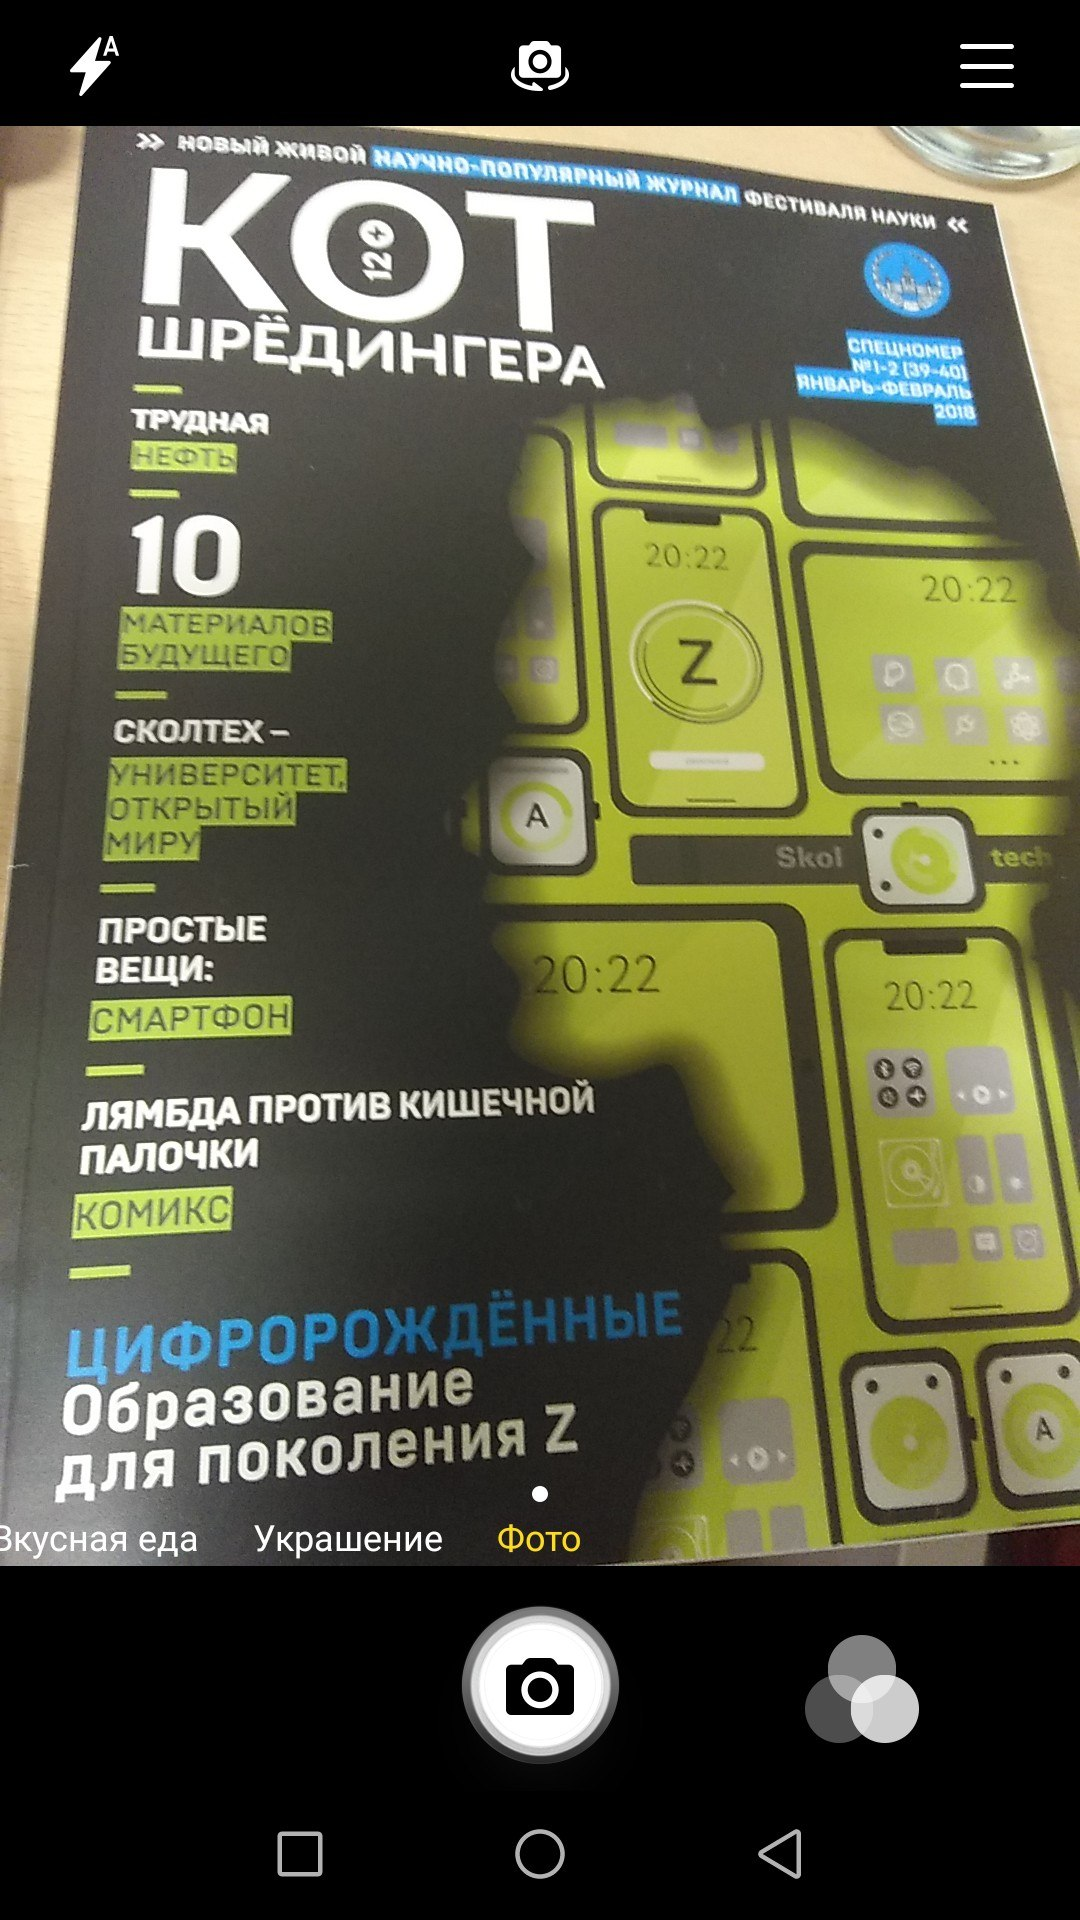
\includegraphics[width=0.4\linewidth]{pics/main}
	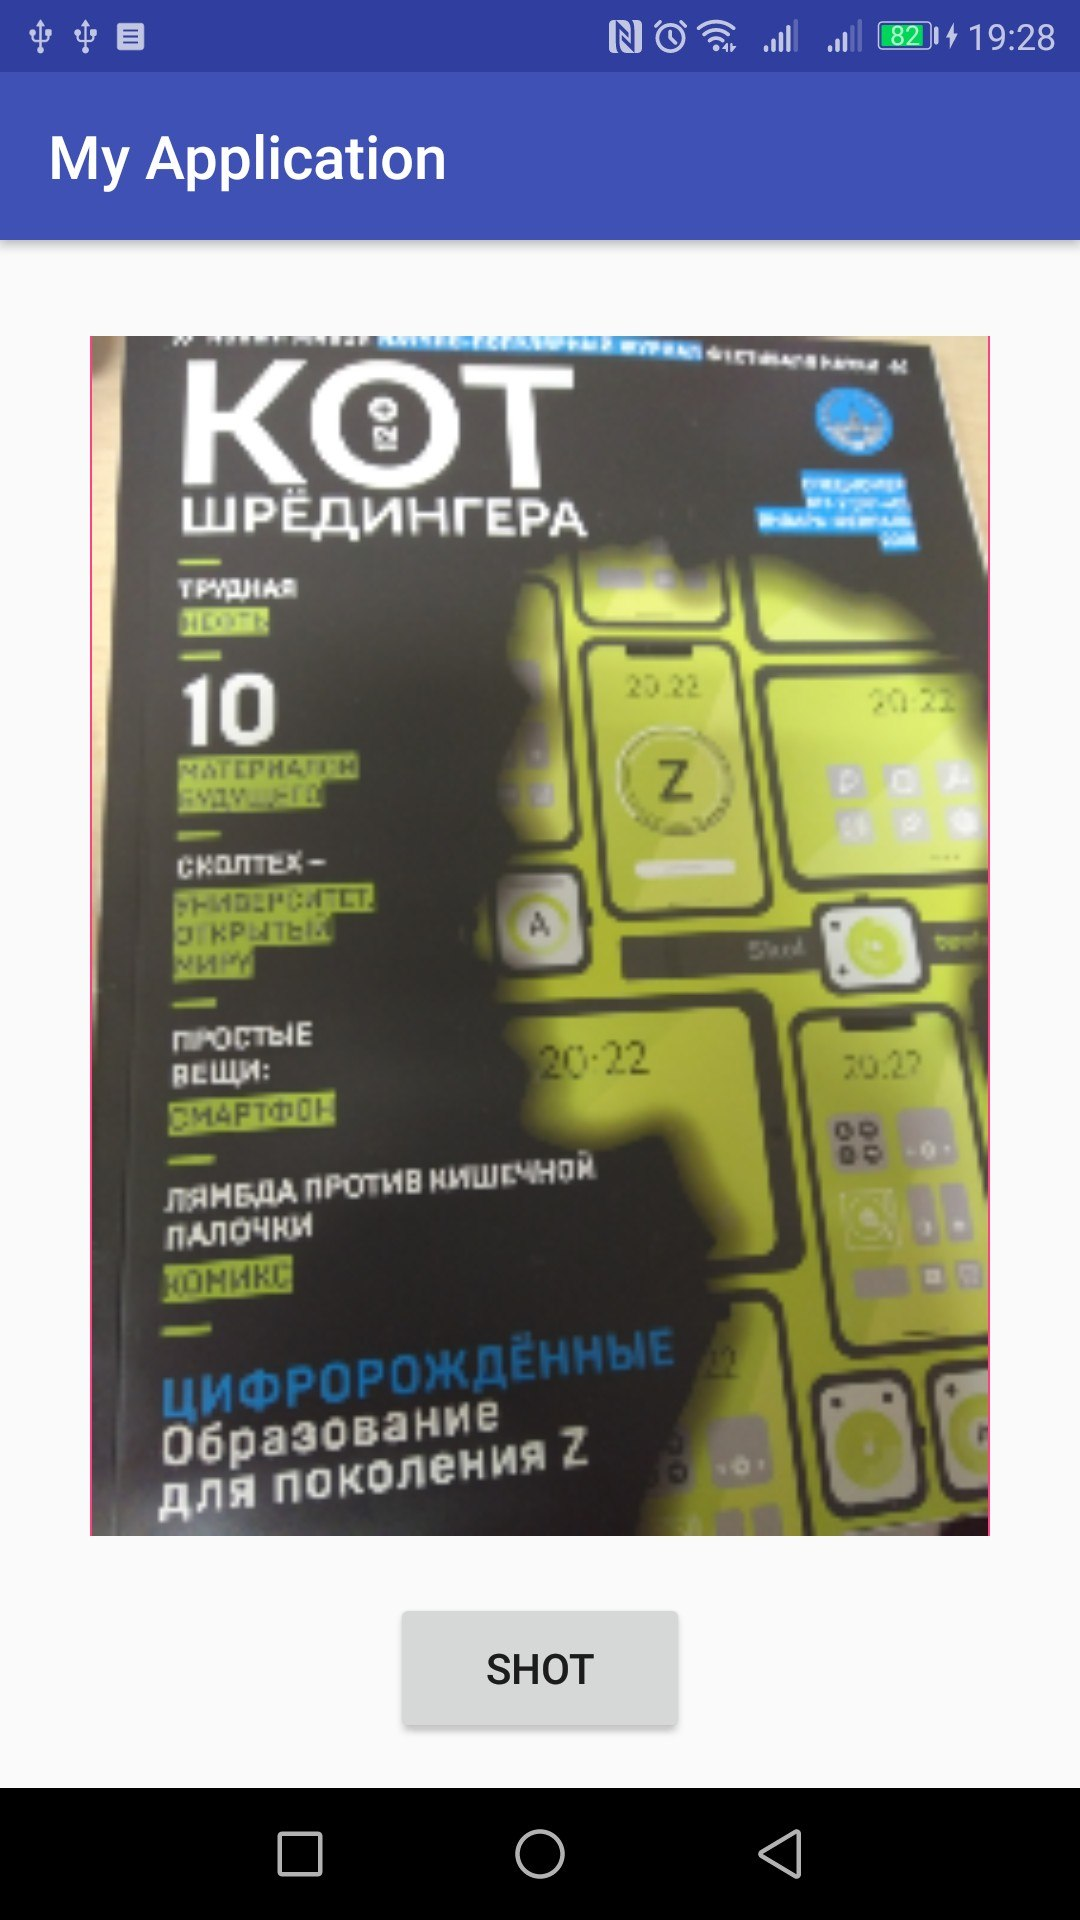
\includegraphics[width=0.4\linewidth]{pics/camera}
	\caption{Результат работы приложения}
	\label{fig:my}
\end{figure}